%%%%%%%%%%%%%%%%%%%%%%%%%%%%%%%%%%%%%%%%%%%%%%%%%%%%%%%%%%%%%%%%%%%%%%%%
%
%		Chapter 5 - Discrete Models
%
%%%%%%%%%%%%%%%%%%%%%%%%%%%%%%%%%%%%%%%%%%%%%%%%%%%%%%%%%%%%%%%%%%%%%%%%


\begin{topic}[Difference Equations]


%\includegraphics*[width=300pt]{images/randomwalk.png}
%
%{\footnotesize (image from \href{https://commons.wikimedia.org/wiki/File:Random_walk_in2D_closeup.png}{Wikimedia Commons} created by Oleg Alexandrov)}
%
%\begin{center}
%	\includegraphics*[width=200pt]{images/SimpleRabbits2.png}
%	
%	{\footnotesize (image from Houman Madani)}	
%\end{center}

\vfil

\begin{center}
\begin{minipage}{300pt}
	\includegraphics*[width=300pt]{images/chap5-xkcd.png}

	\hfill {\footnotesize (image from \href{https://www.xkcd.com/947/}{xkcd - comic \#947})}
\end{minipage}
\end{center}
\end{topic}











%%%%%%%%%%%%%%%%%%%%%%%%%%%%%%
%
%  MODULE - Introduction to Difference Equations
%
%%%%%%%%%%%%%%%%%%%%%%%%%%%%%%



\begin{module}{Introduction to Difference Equations}
	\label{diff:intro}

	In this module you will learn
\begin{itemize}
	\item what is a difference equation
	\item the different types of difference equations
\end{itemize}

\hfill \\[-10pt]


\begin{definition}[Difference Equation]
	A \emph{difference equation} is an equation involving an unknown sequence and a recursive relation between different terms of that sequence.
\end{definition}

\begin{example}
\begin{enumerate}
	\item $u_{k+1} = u_k + u_{k-1}$
	\item $x_k = 2 x_{k-1}$
\end{enumerate}	
\end{example}



Among difference equations, there are lots of types, that require different approaches, so we need to classify them.

\begin{definition}[Types of Differential Equations]
	Just like with differential equations, the main way we distinguish difference equations is according to:
	\begin{itemize}
		\item \emph{order}: the order of a difference equation is the difference between the highest and the smallest terms of the sequence present in the difference equation;
		\item \emph{linear} vs \emph{nonlinear}: A difference equation \quad $F\big(k,u_k,u_{k-1},\ldots,u_{k-n} \big) = 0$ \quad is called \emph{linear} if $F$ is a linear function of $u_k, u_{k-1}, \ldots,u_{k-n}$. Linear difference equations have the form
			$$ a_0(k) u_k + a_1(k) u_{k-1} + \cdots + a_n(k) u_{k-n} = b(k). $$
			All other differential equations are called \emph{nonlinear}.
	\end{itemize}
\end{definition}

\begin{graybox}
	Roughly, to check whether a difference equation is \textbf{linear}, we need to check that:
	\begin{itemize}
		\item The unknown $u_k$ and its other terms appear with exponent 1;
		\item The unknown $u_k$ and its other terms do not multiply by each other;
		\item The unknown $u_k$ and its other terms are not the objects of other functions -- there are no occurrences of things like $\sin(u_k)$ or $e^{u_{k-4}}$, $\ln(u_{k+1})$, $\sqrt{u_{k-1}}$, etc.
	\end{itemize}
\end{graybox}

\begin{example}
\begin{enumerate}
	\item The difference equation $u_{k} = 2 u_{k-2}$ is linear and second-order,because $k-(k-2) = 2$.
	\item The difference equation $u_{k+1} =  u_{k}^2+u_{k-2}$ is nonlinear and third-order, because $(k+1)-(k-2) = 3$.
\end{enumerate}	
\end{example}



Similarly to differential equations, linear difference equations are, in general, easier to study and their theory is much more developed.



%	\begin{exercises}

	\begin{problist}
	\prob Show that all autonomous differential equations are separable.

	\end{problist}
\end{exercises}

\end{module}



\begin{lesson}
	\Title{Introduction to Difference Equations}

	\Heading{Objectives}
	\begin{itemize}
		\item Bla
	\end{itemize}
	
	\Heading{Motivation} 

\end{lesson}


%\newpage
%
%\question
%	Core Exercise with several parts
%\begin{parts}
%	\item Part 1
%	\item Part 2
%\end{parts}
%
%\bookonlynewpage
%
%
%\question
%	One more core exercise
%
%
%
%











%%%%%%%%%%%%%%%%%%%%%%%%%%%%%%
%
%  MODULE - Solving Difference Equations
%
%%%%%%%%%%%%%%%%%%%%%%%%%%%%%%



\begin{module}{Solving Difference Equations}
	\label{diff:solve}

	In this module you will learn
\begin{itemize}
	\item how to solve some types of difference equations
\end{itemize}

\hfill \\


%Let us start with some easier difference equations to gain some intuition on how to solve them.


%\subsection{First-order linear difference equations with constant coefficients}
%
%Let us start with a simple example.
%
%\begin{example}


Let us start with a technique that is very simple and useful, although because it is so simple, it requires some ingenuity to pull off in some cases. \\

\submodule{Expanding to find a pattern} 

We'll start with an example.

\begin{example}
Consider the initial-value problem
$$
\begin{cases}
u_{k+1} = \frac32 u_k & \text{ for } k \geq 0 \\
u_0 = 5	
\end{cases}
$$

Then we can start calculating:
\begin{itemize}
	\item $u_1 = \frac32 u_0 = 7.5$
	\item $u_2 = \frac32 u_1 = 11.25$
	\item $u_3 = \frac32 u_2 = 16.875$
	\item $u_4 = \frac32 u_3 = 25.3125$
	\item $u_5 = \frac32 u_4 = 37.96875$
	\item $\vdots$
\end{itemize}

As you can notice, it's not particularly easy to find a pattern in these numbers. 

The problem is that we \emph{over-simplified}. The trick with this technique is to simplify without over-simplifying.

Let's calculate again:
\begin{itemize}
	\item $u_1 = \frac32 u_0 = \frac32 \cdot 5$
	\item $u_2 = \frac32 u_1 = \frac32 \cdot \frac32 \cdot 5 = \left(\frac32\right)^2 \cdot 5$
	\item $u_3 = \frac32 u_2 = \frac32 \cdot \left(\frac32\right)^2 \cdot 5 = \left(\frac32\right)^3 \cdot 5$
	\item $u_4 = \frac32 u_3 = \frac32 \cdot \left(\frac32\right)^3 \cdot 5 = \left(\frac32\right)^4 \cdot 5$
	\item $u_5 = \frac32 u_4 = \frac32 \cdot \left(\frac32\right)^4 \cdot 5 = \left(\frac32\right)^5 \cdot 5$
	\item $\vdots$
\end{itemize}

Now the pattern should be clear:
$$
u_k = \left(\frac32\right)^k \cdot 5.
$$

To show that this is indeed the solution, we need to use Mathematical Induction (see appendix \ref{app:induction}) to prove it. 
\end{example}

The main idea of this technique is to calculate the terms of the fraction one by one in terms of the initial data.

This is a technique that requires practice, as it is often difficult to judge which parts to simplify and which parts to expand to make sure the pattern emerges clearly. \\

\begin{video}
\begin{itemize}
	\item \qrvideo{https://youtu.be/0OcUAjOXmFc}
\end{itemize}	
\end{video}


\hfill


\submodule{Educated Guessing}

This is the technique we used several times in the book already. We used it with systems of differential equations and with second-order differential equations.

Observe that in the last example, the solution was an exponential, as was the case with differential equations.

\begin{example}
Consider the Fibonacci sequence:
$$
\begin{cases}
f_{k+1} = f_k + f_{k-1} \\
f_0 = 0 \\
f_1 = 1	
\end{cases}
$$

We want to find a formula for $f_k$. To do that, let us assume that the sequence is an exponential. So we can assume that
$$
f_k = r^k,
$$
for some value of $r$.

Let us now use this form of $f_k$ into the difference equation to obtain:
$$
r^{k+1} = r^k + r^{k-1},
$$
which can be simplified by dividing by $r^{k-1}$:
$$
r^2 = r + 1 \quad \Leftrightarrow \quad r^2 - r - 1 = 0.
$$

This is a quadratic equation that we can solve:
$$
r_{\pm} = \frac{1 \pm \sqrt{1 + 4}}{2} = \frac{1 \pm \sqrt{5}}{2}.
$$

So we have two values of $r$ that seem to work. 

That is similar to what we had when solving second-order ODEs (and this is a second-order difference equation).
In that case, the solution turned out to be a linear combination of the two solutions found:
$$
f_k 
	\quad = \quad  c_1 r_-^k + c_2 r_+^k
	\quad = \quad  c_1 \left(\frac{1 - \sqrt{5}}{2}\right)^k + c_2 \left(\frac{1 + \sqrt{5}}{2}\right)^k.
$$

Now we need to find $c_1$ and $c_2$ using the initial data:
\begin{align*}
0 & = c_1 + c_2
	\tag{$k=0$}	 \\
1 & = \quad  c_1 \frac{1 - \sqrt{5}}{2} + c_2 \frac{1 + \sqrt{5}}{2}
	\tag{$k=1$}
\end{align*}
This yields:
\begin{align*}
c_1 & = -\frac{1}{\sqrt{5}}\\
c_2 & = \frac{1}{\sqrt{5}}	
\end{align*}

So the formula we obtain is
$$
f_k =  \frac{1}{\sqrt{5}} \left[\left(\frac{1 + \sqrt{5}}{2}\right)^k - \left(\frac{1 - \sqrt{5}}{2}\right)^k \right].
$$
\end{example}


\begin{important}
The idea of this technique is to assume that the solution is an exponential of the form $r^k$ and find the values for $r$ that solve the particular difference equation. The general solution will be a linear combination of these solutions.
\end{important}

\begin{video}
\begin{itemize}
	\item \qrvideo{https://youtu.be/A5tBvxDM9V4}
\end{itemize}	
\end{video}



	\begin{exercises}

	\begin{problist}
	\prob Consider the initial-value problem
	$$ 	\begin{cases}
			 x_{k+1} = 3 x_k + 4 \\
			 x_0 = 1
 		\end{cases} $$
 	\begin{enumerate}
 		\item Using the expand-until-you-find-the-pattern technique, find the solution of this problem.
 		\item Observe that this problem has an equilibrium solution $x^\star$. What is $x^\star$?
 		\item Define a new sequence $y_k = x_k - x^\star$. Which initial-value problem does ti satisfy?
 		\item Find $y_k$.
 		\item Find $x_k$.
 	\end{enumerate}

	\prob Find the solution to the problem
	$$ 	\begin{cases}
			 x_{k+1} = -2x_{k} +3 \\
			 x_1 = 2
 		\end{cases} $$

	\prob When we were solving ODEs, we considered exponential solutions of the form $u_k = e^{rk}$, but above we considered $u_k = r^k$. Are these equivalent?
	
	Consider the initial-value problem
	$$ 	\begin{cases}
			 x_{k+1} = x_{k} - x_{k-1} \\
			 x_0 = 1 \\
			 x_1 = 2
 		\end{cases} $$

	\begin{enumerate}
		\item Solve the problem assuming the solution is of the form $u_k = r^k$.
		\item Solve the problem assuming the solution is of the form $u_k=e^{rk}$.
		\item What can you conclude?
	\end{enumerate}


	\prob Find the solution to the problem
	$$ 	\begin{cases}
			 x_{k+1} = -2x_{k} - x_{k-1} \\
			 x_0 = 1 \\
			 x_1 = 2
 		\end{cases} $$
	
	\prob Find the solution for the problem
	$$ 	\begin{cases}
			 a x_{k+1} - x_k + (1-a) x_{k-1} = 0 \\
			 x_0 = 1 \\
			 x_N = 0
 		\end{cases} $$
	
	
	\prob Consider the problem
	$$ 	x_{k} - 2x_{k-1}  - x_{k-2} + 2 x_{k-3} = 0 $$
	Find the solution for the following initial conditions.
	\begin{enumerate}
		\item $x_0 = 2, x_1 = 2,	 x_2 = 2$.
		\item $x_0 = 1, x_1 = 0,	 x_2 = 1$.
		\item $x_0 = 1, x_1 = 2,	 x_2 = 3$.
	\end{enumerate}
	
	\prob Consider the problem
	$$ 	\begin{cases}
			 x_{k+1} = -2x_{k} - 2x_{k-1} \\
			 x_0 = 1 \\
			 x_1 = 0 
 		\end{cases} $$
 	\begin{enumerate}
 		\item Find the solution of this problem (it will involve complex numbers).
 		\item Show that $x_k \in \mathbb{R}$ for all $k=0,1,\ldots$
	\end{enumerate}
 	Let us re-write the solution without using complex numbers.
 	\begin{enumerate}[resume]
 		\item Assuming the solution is an exponential $x_k=r^k$, what are the possible values or $r$?
	\end{enumerate}
	This means that the solution is of the form
 		$$ x_k = c_1 r_1^k + c_2 r_2^k.$$
 	We need to know how to easily write $\alpha + i \beta)^k$.
 	\begin{enumerate}[resume]
 		\item Using Euler's Formula in \ref{EulersFormula}, write the complex numbers $r_1$ and $r_2$ in the form
			$$ r_1 = \rho e^{i \theta}.$$
			Also show that 
			$$ r_2 = \rho e^{-i \theta}.$$
		\item Now it should be easier to compute $r_1^k$ and $r_2^k$. After simplifying, use Euler's Formula in \ref{EulersFormula} again to get an expression for $r_1^k$ with $\cos$ and $\sin$.
		\item Let us put everything together again to get a solution of the form
		$$ x_k = a_1 \rho^k \cos(?) + a_2 \rho^k \sin(?).$$
		How do $a_1, a_2$ relate to $c_1,c_2$?
		\item Find the constants $a_1,a_2$.
 	\end{enumerate}
	
	
	\end{problist}
\end{exercises}


\end{module}



\begin{lesson}
	\Title{Solving Difference Equations}

	\Heading{Objectives}
	\begin{itemize}
		\item Bla
	\end{itemize}
	
	\Heading{Motivation} 

\end{lesson}


\newpage


\question	
	Consider the difference equation
	$$	u_{k+1} = 6 u_k - 9u_{k-1}	$$
	
\begin{parts}
	\item Find the solution that satisfies:
		$$ \begin{cases}
			u_0 = 1 \\
			u_1 = 3	
  		\end{cases} $$

	\item Find the solution that satisfies:
		$$ \begin{cases}
			u_0 = 1 \\
			u_1 = 4	
  		\end{cases} $$
\end{parts}



\bookonlynewpage


\question
	Consider a difference equation that has solutions $u_k = r^k$ for $r=2$ and $r=3$.
	
	We also have the conditions:
	$$ 
	u_0 = 0 = 7 \quad \text{ and } \quad u_1=6.
	$$
	
	What is $u_{22}$?




%%%%%%%%%%%%%%%%%%%%%%%%%%%%%%
%
%  MODULE - Modelling with Difference Equations
%
%%%%%%%%%%%%%%%%%%%%%%%%%%%%%%



\begin{module}{Modelling with Difference Equations}
	\label{diff:model}

	In this module you will learn
\begin{itemize}
	\item when to model a quantity using a difference equation instead of a differential equation
	\item different ways to create a model using difference equations
\end{itemize}

\hfill \\

In all the modelling scenarios of chapters 2, 3, and 4, we dealt with continuously changing quantities, and so the appropriate way to model these was through differential equations.

However, not everything changes continuously, somethings change at specific time intervals. For those quantities, differential equations are not the best tool and we turn to difference equations. \\

This module will be divided in several parts depending on the type of situation. \\




\submodule{Economic Models}

Economic quantities often change in bursts, not continuously. That's what happens to a savings account as in the example below, or to stock prices, or to the balance left on a mortgage.
Economic quantities are usually modelled by difference equations.


\begin{example}
We put a certain amount of money in a savings bank account with an annual interest rate of $p\%$, and compounded at regular periods of $\alpha$ (in years).

How does the balance in the savings account change over time? \\

\paragraph{Step 1.} The goal is to model the balance on the account, so define
\begin{itemize}
	\item $b(t)=$ balance on the savings account at time $t$.
\end{itemize}

Notice that the balance on the bank account doesn't change continuously, the balance doesn't change at all until the end of the compounding period. Then the bank adds the interest into the account.

So the balance only changes at each compounding period. We can change our goal to define
\begin{itemize}
	\item $b_n=$ balance on the savings account after $n$ compounding periods.
\end{itemize}


\paragraph{Step 2.} Create a mind map.

We will keep this model simple, so our mind map is just:
\begin{center}
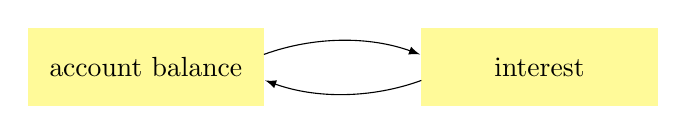
\begin{tikzpicture}
    \fill[color=yellow!40!white] (-4,2) rectangle (-1,3) node[pos=.5] {\color{black}account balance};
%    \draw (-1,2.5) -- (1,2.5);
    \fill[color=yellow!40!white] (1,2) rectangle (4,3) node[pos=.5] {\color{black}interest};
    \draw[-{latex}] (-1,2.66) arc (110:70:2.9);
    \draw[-{latex}] (1,2.33) arc (290:250:2.9);
\end{tikzpicture}	
\end{center}


\paragraph{Step 3.} Let us make the following assumptions:
\begin{itemize}
	\item We make one initial deposit into the account at time $n=0$.
	\item We don't make any more withdrawals or deposits.
	\item The only way the savings account balance changes is through the interest, which is the interest rate $p\%$ of the current balance.
\end{itemize}

\paragraph{Step 4.} We create the following model
$$ 
\begin{array}{ccccccl}
b_{n+1} & = & \big(\substack{\rm previous\\ \rm balance}\big) & + & {\rm interest} \\
b_{n+1}& =& b_n & + & \alpha \frac{p}{100} b_n & = & \left( 1 + \alpha \frac{p}{100}\right) b_n.
\end{array}
$$
	
\end{example}


\hfill

\newpage 
\submodule{Probability Models}

There are several circumstances that involve probabilities that can be modelled using difference equations.

Below is an example of one such circumstance.


\begin{example}

A gambler plays a game at a casino. The game is played one round at a time. 
\vfill

Each round, one of two things happens:
\begin{itemize}
\item The gambler wins \$1 with a probability of $q$
\item The gambler loses \$1 with a probability of $1-q$\\
\end{itemize}

The gambler will stop playing only if
\begin{itemize}
\item The gambler is ruined (bankrupt)
\item The gambler reaches $\$W$.\\
\end{itemize}

What is the probability $\pmb{p_n}$ that the player will be ruined if he starts gambling with $\$n$  ?	 \\


\paragraph{Step 2.} Mind map.
\begin{center}
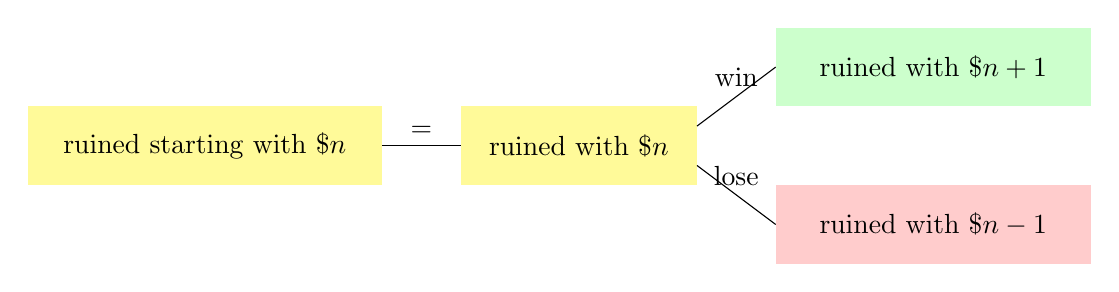
\begin{tikzpicture}
    \fill[color=yellow!40!white] (-4.5,2) rectangle (0,3) node[pos=.5] {\color{black}ruined starting with $\$n$};
    \draw (0,2.5) -- (1,2.5) node[pos=.5,above] {$=$};
    \fill[color=yellow!40!white] (1,2) rectangle (4,3) node[pos=.5] {\color{black}ruined with $\$n$};
    \draw (4,2.75) -- (5,3.5) node[pos=.5,above] {win};
    \fill[color=green!20!white] (5,3) rectangle (9,4) node[pos=.5] {\color{black}ruined with $\$n+1$};
    \draw (4,2.25) -- (5,1.5) node[pos=.5,above] {lose};
    \fill[color=red!20!white] (5,1) rectangle (9,2) node[pos=.5] {\color{black}ruined with $\$n-1$};
\end{tikzpicture}	
\end{center}


The two boxes on the left are very important. The crucial idea is to realize that it doesn't matter when the gambler has $\$n$. If s/he has $\$n$ at two different points in time, then the probability of becoming ruined is the same. \\

This mind map, shows us that we can relate $p_n$, $p_{n+1}$ and $p_{n-1}$.\\

The rest of the modelling will be left as a practice problem.

\end{example}


\begin{video}
\begin{itemize}
	\item \qrvideo{https://youtu.be/Rr2iSKlengg}
\end{itemize}	
\end{video}


\hfill


\submodule{Population Models}

We have modelled populations using differential equations. Populations can be modelled using both differential or difference equations. Which kind of equations to use depends on the goal of the model and the assumptions that we make. 

Below we'll see an example of a population model using difference equations.


\begin{example}

Model a population of mosquitoes, who reproduce at specific times of the year.

\paragraph{Step 1.} The goal is to model the population, so we define
\begin{itemize}
	\item $p(t) = $ population of mosquitoes at time $t$.
\end{itemize}



\paragraph{Step 2.} We create a mind map for this problem.

\begin{center}
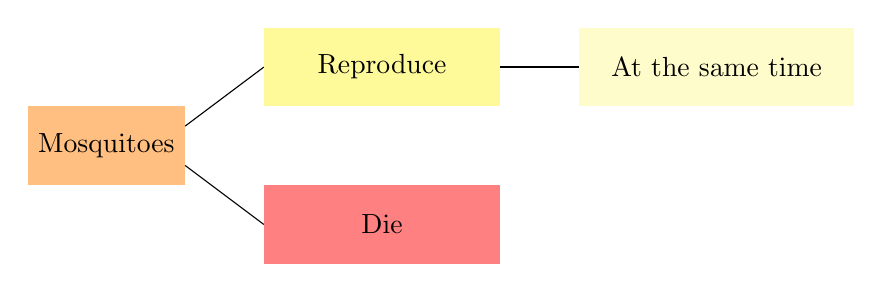
\begin{tikzpicture}
    \fill[color=orange!50!white] (-4.5,2) rectangle (-2.5,3) node[pos=.5] {\color{black}Mosquitoes};
    \draw (-2.5,2.75) -- (-1.5,3.5);
    \fill[color=yellow!40!white] (-1.5,3) rectangle (1.5,4) node[pos=.5] {\color{black}Reproduce};
    \draw (-2.5,2.25) -- (-1.5,1.5);
    \fill[color=red!50!white] (-1.5,1) rectangle (1.5,2) node[pos=.5] {\color{black}Die};
    \draw (1.5,3.5) -- (2.5,3.5);
    \fill[color=yellow!20!white] (2.5,3) rectangle (6,4) node[pos=.5] {\color{black}At the same time};
\end{tikzpicture}
\end{center}



\paragraph{Step 3.} Given that the mosquito population all reproduces at the same time, we don't need to track the population at all times $t$.

So we can assume that the mosquito population doesn't change (much) between seasons, and we change our objective function from $p(t)$ to $p_n$:
\begin{itemize}
	\item $p_n = $ population of mosquitoes at the beginning of season $n$.
\end{itemize}

We understand that mosquitoes die in between seasons, but in this model, we only count the deaths at the beginning of each season. \\

The next assumption is that the number of nymphs (baby mosquitoes) is proportional to the number of mosquitoes in the beginning of the season.

Similarly, the number of deaths is proportional to the number of mosquitoes in the beginning of the season. Also observe that mosquitoes only live for one season, which means that the proportionality constant $\mu > 1$.



\paragraph{Step 4.} So our model is
\begin{itemize}
	\item $p_n = $ population of mosquitoes at the beginning of season $n$.
	\item $p_{n+1} = r p_n - \mu p_n = (r-\mu)p_n$;
	\item $r = $ the average number of nymphs per per mosquito per season;
	\item $\mu = $ the average number of deaths per mosquito per season;
	\item $\mu > 1$, which means that each mosquito itself dies (at the end of the seasons if not earlier), but also some of its nymphs will die.
\end{itemize}

\end{example}

\begin{video}
\begin{itemize}
	\item \qrvideo{https://youtu.be/qmm9GPhA1MY}
	\item \qrvideo{https://youtu.be/j__Kredt7vY}
\end{itemize}	
\end{video}


	\newpage

\begin{exercises}

	Create a model for the following situations.
	\begin{problist}
	\prob You just took a loan to buy a car. You'll need to make fixed payments every period, and the bank will charge an interest on the amount you still owe every period.

		\begin{center}
			\includegraphics*[width=150pt]{images/module25-chirping-echo.pdf}
		\end{center}

	\prob A bird is chirping to find a mate. Unfortunately it is standing next to a cave which echoes its chirps. Consider the following:

 
			\begin{enumerate}[label={(P$_{\arabic*}$) } ]
			\item The bird chirps once every minute;
			\item The maximum volume the bird can chirp is $M$ dB;
			\item If it hears a chirp, then it chirps at a volume proportional to the volume of the chirp it heard times the difference between the maximum volume it is capable and the volume heard with constant $A \ \frac{1}{dB}$;
			\end{enumerate}



	\prob IBM just developed an new software that they wish to charge for usage. In this program, there is a parameter $n$ that you can choose to change how it performs:
			\begin{itemize}
			\item $n^2 = $ number of operations it takes to run the program;
	%		\item Each operation takes $10^{-3}$ seconds;
	%		\item The error of the result is inversely proportional to $n$, i.e., proportional to $\frac1n$;
			\item The profit IBM will make is $- \ln({\rm error})$ in Canadian dollars (negative means that IBM has to pay a penalty).
			\end{itemize}
	
			Model the profit that IBM makes. Remember to consider all sources of costs.
	
	\prob Let us study Engineering students at the University of Toronto. Find a model for the number of undergraduate students in the Engineering school at the University of Toronto and how they change from year to year. 

	\prob You are working for Canada Revenue Agency and the queue in the IRS complaints section is getting too large and lengthy. One way to solve this would be to stop collecting taxes, but that's not possible, so you are tasked with modelling the queue. 

			Model a queue on a typical weekday afternoon minute by minute. 
%			Here are some details about the queue:
%			\begin{itemize}
%			\item The average number of people joining the queue per minute is $\beta$.
%			\item On average, $\gamma\%$ of people in the queue are attended and leave the queue per minute.
%			\item Also on average $\mu\%$ of people in the queue give up waiting and leave the queue per minute.
%			\end{itemize}


	
	\prob Read the example above about the gambler's ruin. Finish creating a model for it.

	\prob A ball bouncing on the floor.
	
	\prob A person has some fever and takes tylenol every 4 hours. What is the concentration of tylenol in her bloodstream?
	
	\end{problist}
\end{exercises}

\end{module}



\begin{lesson}
	\Title{Modelling with Difference Equations}

	\Heading{Objectives}
	\begin{itemize}
		\item Bla
	\end{itemize}
	
	\Heading{Motivation} 

\end{lesson}


\newpage

\question
	Let us expand on the economic example above.
	
	We put a certain amount of money in a savings bank account with an annual interest rate of $p\%$, and compounded at regular periods of $\alpha$ (in years). \\
	
	Even though we call $p\%$ the annual interest rate, because it is compounded during the year, at the end of the year the effective annual interest rate $p_{\rm eff}\%$ is actually higher.
	
	Calculate the effective interest rate $p_{\rm eff}\%$.

\begin{annotation}
\begin{goals}
	The effective annual interest rate is the interest rate with a compounding period of 1 year that gives the same result s the rate of $p\%$ compounded every $\alpha$ years.
\end{goals}
\end{annotation}

	

\bookonlynewpage



\question
	Given a population with
	\begin{itemize}
		\item $\mu=$ probability that an individual will die between two seasons.
	\end{itemize}
\begin{parts}
	\item Define the following quantity
	\begin{itemize}
		\item $P(k)=$probability that an individual born at season $0$ is alive at the beginning of season $k$.
	\end{itemize}
	Find a model for $P(k)$.

	\item What is the probability of the individual dying at age $k$?
	\item What is the average lifespan of an individual in this population?
\end{parts}

\begin{annotation}
\begin{goals}
\begin{itemize}
	\item For the first part, it might be necessary to give the questions:
	\begin{enumerate}[label=(\alph*)]
		\item What is the probability of dying between seasons $(k-1)$ and $k$?
		\begin{itemize}
			\item Find an expression that uses $\mu$.
			\item Find an expression that does not use $\mu$.
		\end{itemize}
	\end{enumerate}
	\item For the last part, the average lifespan is the average of $P(k)$:
	$$ L = \sum_{k=0}^\infty k P(k) $$
	\item Give the hint: $\displaystyle \sum_{k=0}^\infty k r^k = \frac{r}{(r-1)^2}$
\end{itemize}	
\end{goals}
\end{annotation}



\bookonlynewpage


\question
	Consider a population of special rabbits. Once a pair of rabbits is born, they grow and one year later they are still immature. But two years after they are born they give birth to another pair of rabbits.
	
	Model this population of rabbits.
	
	


\bookonlynewpage


\question
	Consider another population of rabbits. This is the lifecycle of a pair of rabbits:
	\begin{enumerate}[label=(year \arabic*)]
		\item Born
		\item Immature (no babies)
		\item Young Adult (2 pairs of babies)
		\item Adult (1 pair of babies)
		\item Old (no babies)
		\item Die
	\end{enumerate}	
	
	Model this population of rabbits.
	
\begin{annotation}
	\begin{goals}
		Students might try to find a pattern. 
		
		It is possible, but very difficult.
		
		Hint: Use a system of difference equations.
	\end{goals}
\end{annotation}
	


%
%
%
%%%%%%%%%%%%%%%%%%%%%%%%%%%%%%%
%%
%%  MODULE - Models with probabilities
%%
%%%%%%%%%%%%%%%%%%%%%%%%%%%%%%%
%
%
%
%\begin{module}{Models with probabilities}
%	\label{diff:prob}
%
%	\input{modules/module23-diff-prob.tex}
%	\input{modules/module23-diff-prob-exercises.tex}
%\end{module}
%
%
%
%\begin{lesson}
%	\Title{Models with probabilities}
%
%	\Heading{Objectives}
%	\begin{itemize}
%		\item Bla
%	\end{itemize}
%	
%	\Heading{Motivation} 
%
%\end{lesson}
%
%
%\newpage
%
%\question
%	Core Exercise with several parts
%\begin{parts}
%	\item Part 1
%	\item Part 2
%\end{parts}
%
%\bookonlynewpage
%
%
%\question
%	One more core exercise
%
%




%
%%%%%%%%%%%%%%%%%%%%%%%%%%%%%%%
%%
%%  MODULE - Models for Two or More Interconnected Quantities
%%
%%%%%%%%%%%%%%%%%%%%%%%%%%%%%%%
%
%
%
%\begin{module}{Models for Two or More Interconnected Quantities}
%	\label{diff:sys}
%
%	\input{modules/module26-diff-sys.tex}
%	\input{modules/module26-diff-sys-exercises.tex}
%\end{module}
%
%
%
%\begin{lesson}
%	\Title{Models for Two or More Interconnected Quantities}
%
%	\Heading{Objectives}
%	\begin{itemize}
%		\item Bla
%	\end{itemize}
%	
%	\Heading{Motivation} 
%
%\end{lesson}
%
%
%\newpage
%
%\question
%	Core Exercise with several parts
%\begin{parts}
%	\item Part 1
%	\item Part 2
%\end{parts}
%
%\bookonlynewpage
%
%
%\question
%	One more core exercise
%
%

%%%%%%%%%%%%%%%%%%%%%%%%%%%%%%
%
%  MODULE - Analysis of Difference Equations
%
%%%%%%%%%%%%%%%%%%%%%%%%%%%%%%



\begin{module}{Analysis of Difference Equations}
	\label{diff:analysis}

	In this module you will learn
\begin{itemize}
	\item some ways to analyze models with difference equations
\end{itemize}

\hfill \\




We have seen some different types of models involving difference equations. we have also seen a few different ways to solve them.

We will now see an example of how we can analyze a difference equation.



\begin{example}

Consider the following model for the number of Mathematics students at a University:
\begin{itemize}
\item $e_k = $ number of students in the year $2020+k$;
\item $a_k = $ number of students admitted to the first year;
\item $g = $ percentage of students that graduate every year;
\item $q = $ percentage of students that quit the Mathematics program  every year. \\

\item $e_{k+1} = e_k + a - g e_k - q e_k$
\end{itemize}

\end{example}

\hfill

\begin{center}
\textbf{\color{cyan}
Finding the equilibrium point(s)
}
\end{center}


What is the equilibrium number of students $E$? This means that we are looking for a solution that remains constant $e_{k+1}=e_k = E$.

$$
E = E + a - (g+q)E
\quad \Leftrightarrow\quad
	E = \frac{a}{g+q}
$$

This is the value that the department should strive for, since it would remain stable.


%\newpage
\hfill

\begin{center}
\textbf{\color{cyan}
Numerical approximations
}
\end{center}


For models with difference equations, we don't need numerical methods, since the recursive definition of the sequence is already a numerical method in itself.

We can follow the same approach however and run some numbers and with different values for the parameters to gain some intuition on the solutions.

\begin{center}
\begin{tabular}{cc}
\includegraphics*[width=150pt]{images/module26-stud-above.png}
	& \includegraphics*[width=150pt]{images/module26-stud-below.png} \\
$e_0 > E$ 
	& $e_0 < E$
\end{tabular}
\end{center}
 

\begin{graybox}
You can access this simulation here:
\begin{itemize}
	\item \qrvideo{https://www.desmos.com/calculator/wv3oxrjvrz}
\end{itemize}	
\end{graybox}


\hfill

\begin{center}
\textbf{\color{cyan}
Qualitative evolution of quantities
}
\end{center}


Let us now look at what happens if the situation is not in equilibrium. The numerical study above, gives some intuition about the behaviour of solutions. 

Let us assume that $e_k  > E$. Then
\begin{align*}
e_{k+1}
	& = e_k (1-g-q) + a \\
	& > E (1-g-q) + a \tag{see note below} \\
	& = E - E(g+q)+a \\
	& = E - \frac{a}{g+q}(g+q) + a\\
	& = E
\end{align*}

\begin{graybox}
\textbf{Note. } This step is only true if $E$ and $1-g-q>0$. (Why?) \\

It's clear that $E$ should be positive, since it is a number of students. \\

The other quantity is not so obvious: \quad $g+q < 1$ ?

In fact, $g+q$ is the fraction of students that graduate or quit the Mathematics program, so it can't exceed 1! (Why?)
\end{graybox}


We conclude that if $e_k > E$, then $e_{k+1}>E$. This means that if the number of students starts above the equilibrium, then it will always stay above it.\\

But will the number of students keep increasing without bound or will it converge to a number?\\

Let us check:
\begin{align*}
e_{k+1} - e_k
	& = a - e_k (g+q) \\
	& < a - E (g+q) \\
	& = a - \frac{a}{g+q} (g+q) \\
	& = 0
\end{align*}

So we conclude that 
$$
e_{k+1} - e_k < 0 \quad \Leftrightarrow \quad e_{k+1} < e_k,
$$
so the number of students will decrease.

Our conclusion is that if $e_k > E$, then $e_{k+1} \in [E, e_k]$:
\begin{center}
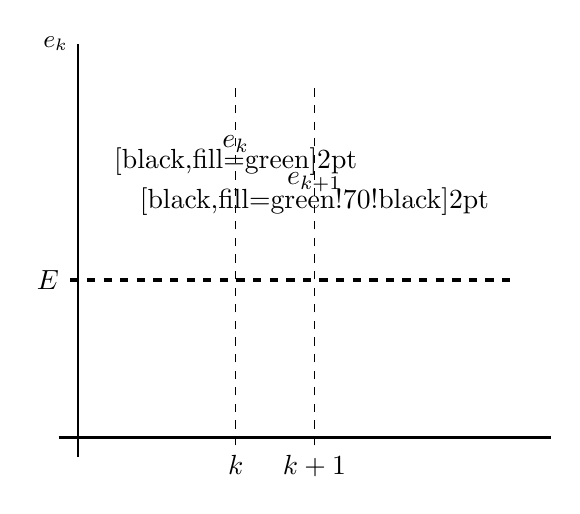
\begin{tikzpicture}
  \draw[thick,-{\seta}] (-0.25,0) -- (6,0) ;%node[above] {\small $k$};
  \draw[thick,-{\seta}] (0,-0.25) -- (0,5) node[left] {\small $e_k$};
%  \draw[] (2,0) node[below] {$k$};
  \draw[dashed] (2,-0.1) node[below] {$k$} -- (2,4.5);
%  \draw[] (3,0) node[below] {$k+1$};
  \draw[dashed] (3,-0.1) node[below] {$k+1$} -- (3,4.5);
  \draw[ultra thick,dashed] (-0.1,2) node[left] {$E$} -- (5.5,2)  ;
%
  \draw (2,3.5) node {\tikzcircle[black,fill=green]{2pt}} node[above] {$e_{k}$};
  \draw (3,3) node {\tikzcircle[black,fill=green!70!black]{2pt}} node[above] {$e_{k+1}$};
\end{tikzpicture}
\end{center}


Similarly, if $e_k < E$, we can conclude that $e_{k+1} \in [e_k,E]$:
\begin{center}
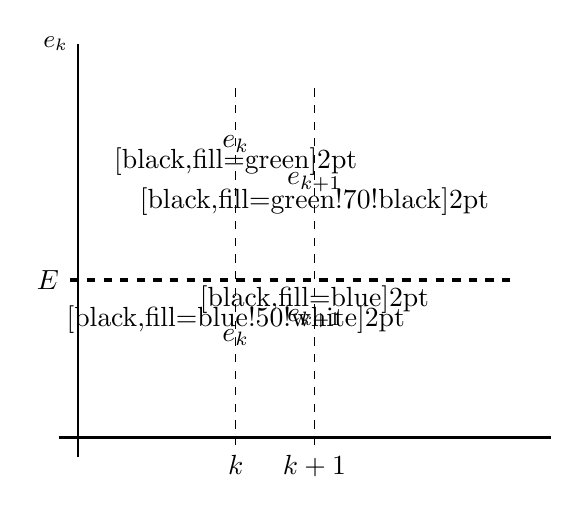
\begin{tikzpicture}
  \draw[thick,-{\seta}] (-0.25,0) -- (6,0) ;%node[above] {\small $k$};
  \draw[thick,-{\seta}] (0,-0.25) -- (0,5) node[left] {\small $e_k$};
%  \draw[] (2,0) node[below] {$k$};
  \draw[dashed] (2,-0.1) node[below] {$k$} -- (2,4.5);
%  \draw[] (3,0) node[below] {$k+1$};
  \draw[dashed] (3,-0.1) node[below] {$k+1$} -- (3,4.5);
  \draw[ultra thick,dashed] (-0.1,2) node[left] {$E$} -- (5.5,2)  ;
%
  \draw (2,3.5) node {\tikzcircle[black,fill=green]{2pt}} node[above] {$e_{k}$};
  \draw (3,3) node {\tikzcircle[black,fill=green!70!black]{2pt}} node[above] {$e_{k+1}$};
  \draw (2,1.5) node {\tikzcircle[black,fill=blue!50!white]{2pt}} node[below] {$e_{k}$};
  \draw (3,1.75) node {\tikzcircle[black,fill=blue]{2pt}} node[below] {$e_{k+1}$};
\end{tikzpicture}
\end{center}


So we can see that the sequence $e_k$ will be approaching $E$, so we can say that the \emph{equilibrium is stable}.







\hfill

\begin{center}
\textbf{\color{cyan}
Limiting behaviour of the solutions
}
\end{center}



From our previous analysis, we can see that it looks like 
$$
\lim_{k \to \infty} e_k = E.
$$

But we didn't prove this yet. It could be that the sequence converges to some other value. 

To show this, we would need to define a new sequence $x_k = e_k-E$, assume that it has the form $x_k = C r^k$ and then obtain a characteristic equation for $r$:
$$
r = 1-g-q \in (0,1),
$$
so $x_k = C r^k$ and 
$$
\lim_{k \to \infty} x_k = 0
\quad \Leftrightarrow \quad
	\lim_{k \to \infty} e_k = E.
$$

So we now know that the number of students will converge monotonically to the equilibrium.








	\newpage 

\begin{exercises}

		\begin{problist}
	
	\prob Consider the following discrete population model:
	\begin{itemize}
		\item $p_k=$ population at the beginning of season $k$
		\item $R = $ basic reproduction value for the population
		\item $K= $ carrying capacity 
		\item $\displaystyle p_{k+1}=p_k + R p_k\left(1-\frac{p_k}{K}\right)$
	\end{itemize}
	
	\begin{enumerate}
		\item Define:
		\begin{itemize}
			\item $\mu = 1+R$,
			\item $\displaystyle x_k = \frac{R}{1+R} \frac{p_k}{K}$.
		\end{itemize}
		Show that $x_{k+1} = \mu x_k (1-x_k)$.
		\item What are the equilibrium values for $x_k$?
	%	$$
	%	E = 1 - \frac1\mu = \frac{mu-1}{\mu}
	%	$$
	
		\item Take $R=1, \mu=2$. Compare this model with the continuous logistic model.
		\item In the continuous model, solutions cannot cross the equilibrium. 
		Change the value of $R,\mu$ and show that in this discrete model, solutions can cross the equilibrium.
		
		\item Take $R=3, \mu=4$ (constants for influenza virus). Below is a graph with $\color{green!70!black}x_0 = 0.1$ and $\color{blue!85!black}x_0=0.101$.
	
			\begin{center}
				\includegraphics*[width=150pt]{images/module26-logistic.png}
			\end{center}
		
			Which conclusions do you take from this graph?
			
		\item Take $x_0=\frac12$. What happens to $x_k$ as $k$ gets larger and larger: does it remain bounded, or does it converge to $\pm \infty$? Check for different values of $\mu$.

		\item You'll need to program for this exercise. Now allow complex values for $\mu \in \mathbb{C}$. In a graph, mark the values of $\mu \in \C$, for which $x_n$ does not diverge to infinity.
		
%		\includegraphics*[width=150pt]{images/module26-mandelbrot.png}
		
	\end{enumerate}

\begin{annotation}
\begin{goals}
	\begin{itemize}
	\item[1.] You can skip the first part and tell students to do it at home.
	
	\item[3.] For the comparison part, notice how the model is very similar in the way it looks. If you run the model it also behaves very similarly.

	\qrvideo{https://www.desmos.com/calculator/zxk8udxmac}
	
	\item[4.] For the last part, for $\mu=3$, solutions oscillate but converge to equilibrium
	\item[5.] For the last part, for $\mu=4$, $x_0=0.1$ and $x_0=0.101$ gives completely different solutions. Chaotic behaviour. So need to be careful analyzing nonlinear difference equations.
	
		\qrvideo{https://www.desmos.com/calculator/e656u8n4vt}
	\end{itemize}
\end{goals}	
\end{annotation}

	

	

	\prob Consider the model for a queue:
	\begin{itemize}
		\item $q_n=$ number of people waiting in the queue at minute $n$;
		\item $\gamma=$ fraction of the people waiting that are attended each minute;
		\item $\mu=$ average number of people that give up waiting in the queue per minute;
	\end{itemize}

	\begin{enumerate}
		\item First, let us find out a very bad scenario for the queue. Find a number of initial people in the queue $q_0$ such that the size of the queue will never change.
		\item Let 
			\begin{itemize}
				\item $p_k=$ probability that a person who joined the queue at time $k=0$ will still be waiting after $k$ minutes.
			\end{itemize}
			Is $p_k$ increasing, decreasing, or not monotone?
		\item The probability that someone waited exactly $k$ minutes is $p_{k}-p_{k+1}$.
			Find another expression for $p_{k}-p_{k+1}$ without using $p_k$.
		\item The expected waiting time in the queue is given by the ``law'':
			
			\hspace{-.05\textwidth}\framebox{
			\begin{minipage}{.4\textwidth}
			The expected waiting time is the weighted average of the possible waiting times, where the weights are the probability of waiting that exact amount of time.
			\end{minipage}}
			
		Find the expected waiting time for this queue.
	\end{enumerate}
	
	
	
	
	
	\prob 	Two computers are facing each other on video conferencing software. The first computer makes a sound and every fraction of a second, the other computer reproduces the sound.
	
	Consider the following model for the microphone feedback:
	\begin{itemize}
		\item $v_n =$ volume produced by the first computer (in dB) for the $n$ iteration;
		\item $e=$ fraction of the original volume reproduced by the second computer;
		\item $M=$ maximum volume that first computer can produce (in DB). \\

		\item $v_{n+1} = e v_n \left( \frac{M - e v_n}{M}+1\right)$.
	\end{itemize}
	
	\begin{enumerate}
		\item What is the initial volume that will just cause the following iterations to be the same?


		\item Find a condition on $e$ that allows for the previous situation to occur.

%v>0 iff 
%v<M iff 

		\item Assume $e \in (0,1)$. What happens if the initial volume is softer than the equilibrium? What happens if the initial volume is louder than the equilibrium?
		\item Assume $e>1$. What happens if the initial volume is softer than the equilibrium? What happens if the initial volume is louder than the equilibrium?

		\item Assume $e=\frac85$. Sketch a graph of the solution.
		
%		\begin{itemize}
%			\item $v_0 = M$	
%			\item $v_1 = \frac{16}{25}M$
%			\item $v_2 = \frac85 \frac{16}{25}M \frac{122}{125} \approx M$
%		\end{itemize}

		What is the behaviour of the solution as $n$ gets larger?
		
		\item Assume $e=\frac{1+\sqrt{5}}{2}$ the golden ratio. Is there an initial volume that gives a periodic solution: $v_0=v_2=v_4,v_5=\cdots$ and $v_1=v_3=v_5=v_7=\cdots$?
	
	\end{enumerate}
	
\begin{annotation}
\begin{goals}
	For 2, remember that the first computer has to be able to produce the sound: $v_n < M$, and the sound needs to be audible $v_n>0$.
\end{goals}	
\end{annotation}


		
	\end{problist}
\end{exercises}
\end{module}



\begin{lesson}
	\Title{Analysis of Difference Equations}

	\Heading{Objectives}
	\begin{itemize}
		\item Bla
	\end{itemize}
	
	\Heading{Motivation} 

\end{lesson}


\newpage

\question
	Core Exercise with several parts
\begin{parts}
	\item Part 1
	\item Part 2
\end{parts}

\bookonlynewpage


\question
	One more core exercise




%
%
%%%%%%%%%%%%%%%%%%%%%%%%%%%%%%%
%%
%%  MODULE - Nonlinear Models
%%
%%%%%%%%%%%%%%%%%%%%%%%%%%%%%%%
%
%
%
%\begin{module}{Nonlinear Models}
%	\label{diff:nonlinear}
%
%	In this module you will learn
\begin{itemize}
	\item some nonlinear models
	\item some of the difficulties of studying nonlinear models
\end{itemize}

\hfill \\


%	\begin{exercises}

	\begin{problist}
	\prob Show that all autonomous differential equations are separable.

	\end{problist}
\end{exercises}

%\end{module}
%
%
%
%\begin{lesson}
%	\Title{Nonlinear Models}
%
%	\Heading{Objectives}
%	\begin{itemize}
%		\item Bla
%	\end{itemize}
%	
%	\Heading{Motivation} 
%
%\end{lesson}
%
%
%\newpage
%
%\question
%	Core Exercise with several parts
%\begin{parts}
%	\item Part 1
%	\item Part 2
%\end{parts}
%
%\bookonlynewpage
%
%
%\question
%	One more core exercise
%
%

